%! TEX root = 'main.tex'
\section{Background and Adversary Model}
\label{sec:background}

In this section, we provide basic knowledge for the rest for the rest of the paper. We provide detailed information about industrial control systems(ICS) and programmable logic controllers(PLC), and we define the adversary model we will introduce throughout the paper.

\subsection{Background}

An ICS is a distributed system which is composed of physical components, like sensors and actuators, which interact with the physical system (e.g., power grid) and cyber components(e.g., cyber-networks and servers). Although ICS are largely self-contained, interfaces exist through which external components can interact with the systems. For instance, a human operator can monitor the systems state and influence it through a human-machine interface(HMI). Most PLCS are connected to the ICS via an Ethernet network, and hence, often indirectly connected to the Internet. It is also quite common that PLCs are directly connected to the Internet. 

Centralized operation and maintenance is an essential feature of ICS. An operator can program and monitor PLCs and the applications running on them remotely, i.e., retrieve the status of a PLC and re-program it over the network. The information which can be retrieved from the PLC contains, among others, the control logic application on the PLC. All applications, including their source code and further meta information, can be loaded from a PLC.

Essentially, ICS is equivalent to a large computer networks. Two points make it special. First, instead of personal computers or enterprise servers, ICS usually controls vital infrastructures of nation, such as power grid. The recent incident of new york and south American cities blackout shows the importance to the stability of societies.

Second, ICS use special purposed devices such as Programmable Logic Controllers(PLC). Unlike PC and smart phones  which mostly adopt x86 and ARM architecture with well defined peripheral device protocols and well-know operating systems such as Windows and Linux/Unix, each PLC manufacture may use different architecture, some of them may even be proprietary design, with unknown system bus and peripheral devices. Moreover, their is no unified operating system for different brand PLCs, there programming languages are also different.


\textbf{Programmable Logic Controllers(PLC).} Programmable logic controller are cyber-physical systems that are used to control industrial appliances. PLCs have input and output modules to interact with the physical world. They can translate physical inputs, mostly current on a wire, into digital values and vice versa. Connected to physical appliances such as sensors and actuators, PLCs can convert sensor readings into digital values, process the readings with the build-in computing unit, and forward the outputs to the physical world. The logical behavior of PLCs, i.e., the processing of the input data, is programmable.

Such protocol loops can be either local, i.e., the inputs and outputs are handled by a single PLC, or distributed, i.e., the inputs are read by one PLC and forwarded over the network to another PLC.

The two main software components of a PLC, control logic and firmware. The firmware is acting as a kind of operating system(OS). The firmware contains, among other functionality, modules to read and write the inputs and outputs of the PLC from/to the physical world. These modules can be seen as drivers for the I/O hardware. Control programs can be considered the PLC's application layer. For instance, ladder logic is commonly used in PLCs, it adopts a visual way to express how the industrial control logic should perform among conditions and devices. Later it will be compiled into the native binary and sent to firmware to load and run. The ladder logic programs are executed repeatedly in fixed intervals, called scan cycles. It reads data from firmware routines, compute/analysis and then send the result back. That's the software part. A PLC device normally have wire sockets and LEDs as indicator, although it has network connection that allows it to transfer current status back to Supervisory Control and Data Acquisition(SCADA), but to the physical world, the input/output wires are the main way to control. When the ladder logic calling firmware routines to toggle a trigger, this operation will be transferred to setting/clearing a memory cell. Eventually, the microcontroller in the PLC set 0 or 1 on the corresponding general purpose input/output(GPIO) pin. And this pin goes through extra circuity such as output buffer to the outside wire.   






\subsection{Adversary Model}
In general, to compromise an industrial control system, attacks could been categorized into two basic groups. Software exploitation and hardware manipulation.

\textbf{Software Exploitation.} Many attacking surfaces exist in this category. In the past, due to the lack of security measure, attackers can connect to PLC and use the existing mechanism to load a new ladder logic or module to run, \textcolor{red}{cite simens}. Or, there are many network faced services such as CAN bus or a web portal may potentially have vulnerability in their implementation. By exploiting the vulnerabilities, attackers could first win part of the PLC and then further gain control of the real-time microcontroller which directly controls the physical industrial devices \textcolor{red}{cite simens}. These type of attack is straight forward and effective. But the problem is that direct network access is required. Network isolation is a common practice in vital industrial systems. It's still possible to make a successful attack, for instance, the infamous Stuxnet. The Stuxnet virus used several 0day exploits and had a  penetration plan, and it actually took years to spread a virus and finally located the target network. On the other hand, many research focus on this and mitigations start to get applied, which makes direct software exploit more and more difficult. Naturally, leaving preset backdoors in firmware and hardware starts to draw attackers attention.  


\textbf{Hardware manipulation.} Hardware attacks are easily related to supply chain security. Every node in the supply chain can be infiltrated and exploited by attackers. Chip design modification is the most stealthy one, but it's hard due to the fact that there are only few microchip fabrication plant can produce certain type of microcontroller or SoC. Lower in the supply chain where the PLC is manufactured and assembled, it's more practice. Detecting a supply chain compromise is a difficult and costly endeavor. This requires strict security and quality control throughout every phase of the supply chain even including shipping.

Firmware modification attacks is effective, even with some lightweight checksum and encryption scheme which can be bypassed. But, if the hardware keeps integrity, then the malicious firmware could be find out by software auditing such as a firmware image trust list.

Hardware have some advantages. When looked at a PCB board of PLC, mostly the electronic design, wire routing is not intuitive for most of the users. Several layers of PCB contains hundreds of wires connecting dozens of chips. And, for each chip, we tend to believe what it prints on the surface. There is no easy to verify the functionality of each chip to what it claims. As mentioned earlier, all the software level logic, to the physical systems, eventually ends up as signals on the GPIO pins. Changing the voltage levels on the wires severs the purpose of controlling industrial devices as what software ladder logic does. There are different peripheral protocols and buses in a PLC, each of them plays different roles in the system. For example, in order to send in data, some flash chip could use SPI as the protocol to communicate with the microcontroller. Tapping on the SPI wires, the malicious circuit could change the data that being transferred. In this paper, we choose a very common interface called JATG as the main carrier of our malicious operations.   

JTAG is is an industry standard for verifying designs and testing printed circuit boards after manufacture. Among various components and buses on a PCB board, JTAG is low speed and it can reach a wide range of the system. Multiple chips can be daisy chained together. This type of setup allows one set of JTAG interface to control multiple devices.

We prototyped a device which is small enough to mount on the PCB board of a PLC. This could happen inside the supply chain, any one with physical access to a PLC could easily open the case and mount the hardware implant.

We also propose a more stealthy way detailed in Further Work section.



\subsection{JTAG}
JTAG interface named after Joint Test Action Group, is a industry standard port for IC testing. This is necessary because of the growing complexity of integrated circuits makes the design verification tends to be more and more difficult.

The JTAG interface use very few pins (TDI, TDO, TMS and TCK) to talk to test access port(TAP) which implements a state machine and a set of registers to further connect more circuit components, from which it can access memory bus and more debug facilities, as shown in ~\autoref{fig:jtagsm}. The two major register of TAP are Instruction Register(IR) and Data Register(DR). They work in a serial mode in which they accepts/sends out bit stream through the four former mentioned JTAG pins. The IR register contains the command to be executed, DR contains shift-in data or the command's result. JTAG is just a way to read/write data to different registers/components that connected to the system. It's early applications targeted board level testing, diagnosis and fault isolation. Nowadays JTAG is used as the primary way of accessing sub-blocks of integrated circuits, making it the most common way to debug embedded system. In this project, the PLC we work with use ARM cortex-m3 based microcontroller, ARM Cortex-M series  contains CoreSight Technology which is a power debug model. The CoreSight can't be operated through either JTAG or SWD(Serial Wire Debug) interface.

\begin{figure}[th]
	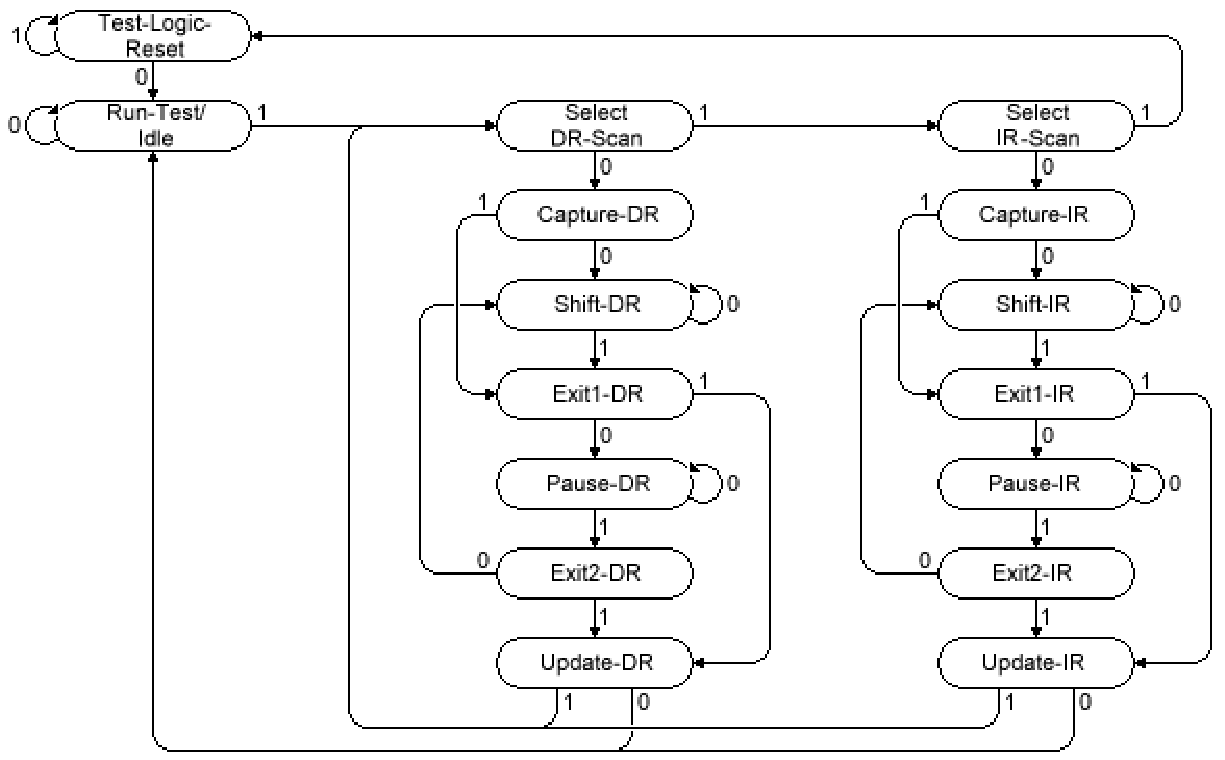
\includegraphics[width=0.47\textwidth]{figures/jtagsm}
	\centering
	\caption{JTAG TAP state machine.}
	\label{fig:jtagsm}
\end{figure}


On ARM Cortex-M series microcontroller has build on a Debug Access Port(DAP) which is comprised of a Debug Port(DP) and several Access Ports(AP). DP manages the connection to an external debugger. APs access on-chip system resources. DAPBUS connects the DP to one or more APs. The APs provide non-invasive access to APB bus though APB-AP,  and to other legacy-configured debug components using JTAG-AP. In our project, we access system memory and memory-mapped IO through AHB-AP. Because of this comprehensive debug ability that ARM provide, our hardware implant can fully control the system by connects to the JTAG pins.

On the real-time microcontroller board, we found JTAG solder joints, as shown in~\autoref{fig:board_jtag}. It supports both JTAG and SWD (Serial Wire Debug\cite{ashfieldserial}) interfaces. In this paper, we choose to use JTAG interface. But if you use the SWD interface, some of the pins will be reused as SWD pins. 

\begin{figure}[th]
	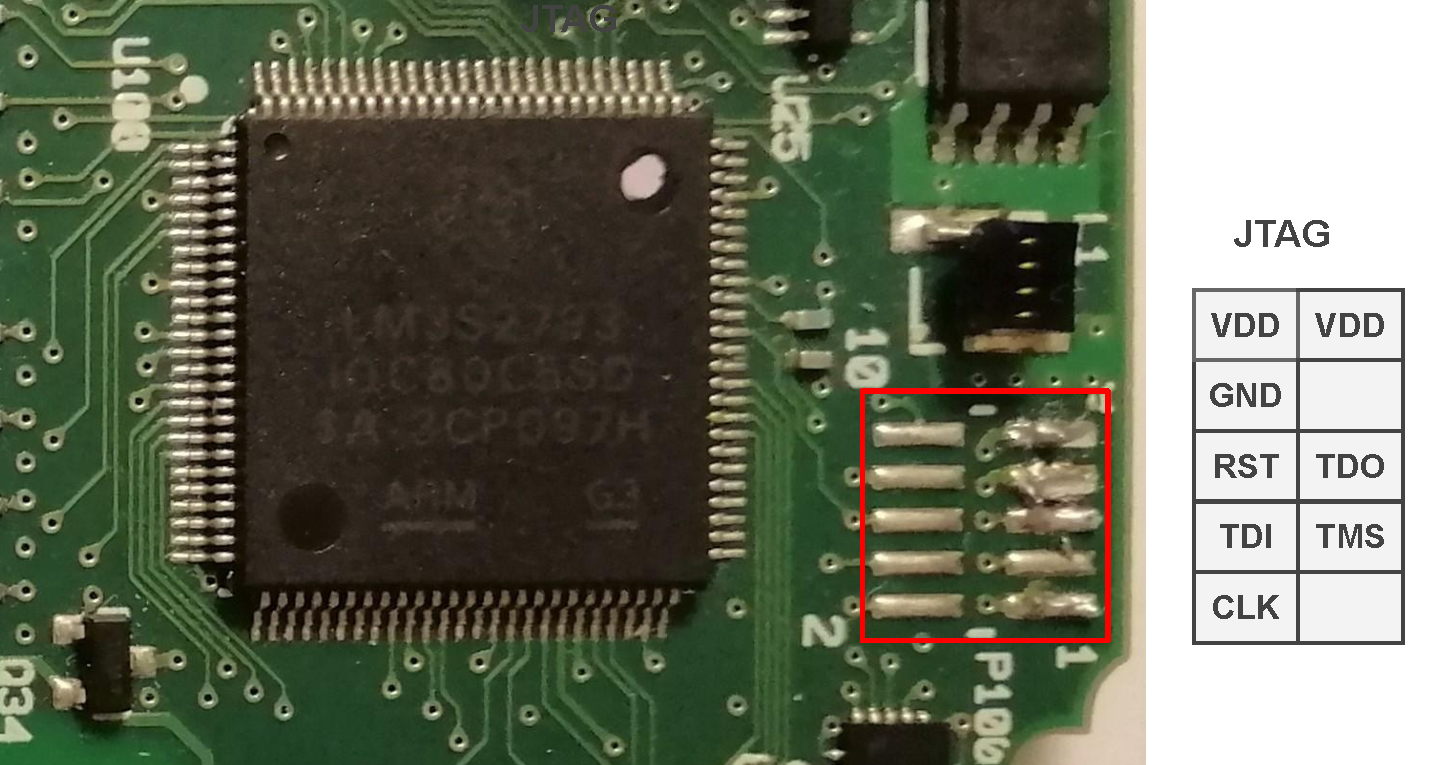
\includegraphics[width=0.47\textwidth]{figures/board_jtag}
	\centering
	\caption{JTAG Interface on the Real-time Microcontroller Board}
	\label{fig:board_jtag}
\end{figure}

The JTAG specification allows for several devices to be connected to a single interface in a daisy chain configuration. In this case, we found that there is only one microcontroller connected.

Because we want to implement JTAG debugging functionality on a very small device, in order to be able to fit into the PLC case. Currently we choose Teensy 3.2 development board. For smaller PCB boards, smaller chips are required, such as an 8-bit microcontroller system, which typically has very limited on-chip memory. So we choose to implement the JTAG driver ourselves, instead of choosing an open source project, such as OpenOCD\cite{hogl2006open}. The code for implementing JTAG debugging with Teensy 3.2 development board has been uploaded to github\footnote{https://github.com/whensungoesdown/teensyi\_jtag}. It only needs to modify 4 GPIO pins, so it can be easily ported to other devices.
